\documentclass{article}
\usepackage{graphicx}        % 插入图片
\usepackage{ctex}            % 支持中文
\usepackage{authblk}         % 作者和单位信息
\usepackage{abstract}        % 摘要格式
\usepackage{titling}         % 标题格式自定义
\usepackage{multicol}        % 多栏排版
\usepackage{geometry}        % 页面布局设置
\usepackage{gbt7714}         % 国标参考文献格式
\usepackage{amsmath}         % 数学公式
\usepackage{fontspec}        % 英文字体设置
\usepackage{xcolor}          % 颜色定义
\usepackage{capt-of}         % 双栏环境图片标题
\usepackage{titlesec}        % 章节标题格式
\usepackage{caption}         % 图表标题格式
\usepackage{threeparttablex} % 带注释的表格
\usepackage{booktabs}        % 专业表格线条
\usepackage{array}           % 表格列宽调整
\usepackage{longtable}       % 跨页表格
\usepackage{fancyhdr}        % 页眉页脚设置
\usepackage{setspace}        % 行间距设置
\usepackage{hologo}          % 中文参考文献格式修正

% 颜色定义 - 主色调
\definecolor{mycolor}{rgb}{0,0.28,0.6}

% 字体设置
\setmainfont{Times New Roman} % 英文字体
\newcommand{\customsectionformat}{\zihao{4}\songti}      % 一级标题格式:四号宋体
\newcommand{\customsubsectionformat}{\zihao{5}\heiti}    % 二级标题格式:小五号黑体
\newcommand{\customsubsubsectionformat}{\zihao{5}\kaishu} % 三级标题格式:小五号楷书

% 章节标题样式设置
\titleformat{\section}{\normalfont\customsectionformat\color{mycolor}}{\thesection}{1em}{}
\titleformat{\subsection}{\normalfont\customsubsectionformat\color{mycolor}}{\thesubsection}{1em}{}
\titleformat{\subsubsection}[runin]{\normalfont\customsubsubsectionformat\color{mycolor}}{\thesubsubsection}{1em}{}

% 页面边距设置
\geometry{headsep=0.5cm}
\geometry{left=25mm,right=25mm,top=28mm,bottom=30mm}

% 页眉页脚设置
\pagestyle{fancy}
\fancyhf{}
\chead{{\zihao{-5}\songti 这里是页眉文章标题}}
\rhead{\thepage}
\renewcommand{\headrulewidth}{0.5pt}
\fancypagestyle{plain}{\pagestyle{fancy}}

% 自定义样式 
\fancypagestyle{mystyle}{
    \chead{{\zihao{-5}\songti 中山大学学报(自然科学版)}\par\noindent ACTA \; SCIENTIARUM \; NATURALIUM \; UNIVERSITI \; SUNYATSENI}
    \rhead{\thepage}
    \lfoot{\zihao{-5} \heiti 作者简介:\songti 你的名字(2006年生),男;\heiti 研究方向:\songti 目标检测;E-mail:your\_ name@mail2.sysu.edu.cn}
    \renewcommand{\headrulewidth}{0.5pt}
    \renewcommand{\footrulewidth}{0.5pt}
}

% 标题格式优化 - 减少标题周围的空白
\makeatletter
\def\@maketitle{%
  \newpage
  \null
  \vskip 0.5em% 标题上方留白
  \begin{center}%
    {\LARGE \@title \par}%
    \vskip .5em% 标题和作者之间的留白
    {\large \linespread{1.3}\@author \par}%
    \vskip 1em% 作者和日期之间的留白
    {\large }%
  \end{center}%
  \par
  \vskip 1.5em}
\makeatother

% 参考文献设置
\ctexset{bibname=\zihao{5} 参考文献:} % 参考文献标题格式

\begin{document}

% 标题、作者和单位信息
\title{\zihao{2}\songti \color{mycolor}{\textbf{这里是文章标题}}}
\author{\zihao{4}\kaishu\color{mycolor} {Wenjie Shi}}
\affil{\zihao{5}\kaishu 中山大学智能工程学院,广东 \ 深圳518107}
\date{}

\maketitle
\thispagestyle{mystyle}
\ziju{0.085} % 字间距

% 摘要和关键词
\noindent
\zihao{-5}\heiti {\textbf{摘 \ \  要}}:\zihao{-5}\songti{
随着深度学习在该领域的广泛应用,目标检测技术在灵活性、效率和准确性上不断进步。}

\noindent
\zihao{-5}\heiti{\textbf{关键词}}:\zihao{-5}\songti{深度学习;目标检测}

% 设置双栏布局
\setlength\columnsep{0.8cm} % 双栏间距
\begin{multicols}{2}

\section{ 引 \ 言}
\zihao{5}\songti  % 正文使用小五号宋体
这不是官方模板,是我参考官方word模板自制的latex模板,与官方模板可能不能完全一样,仅为写作业使用。

% 跨双栏的大图示例
\begin{figure*}[t]
    \centering
    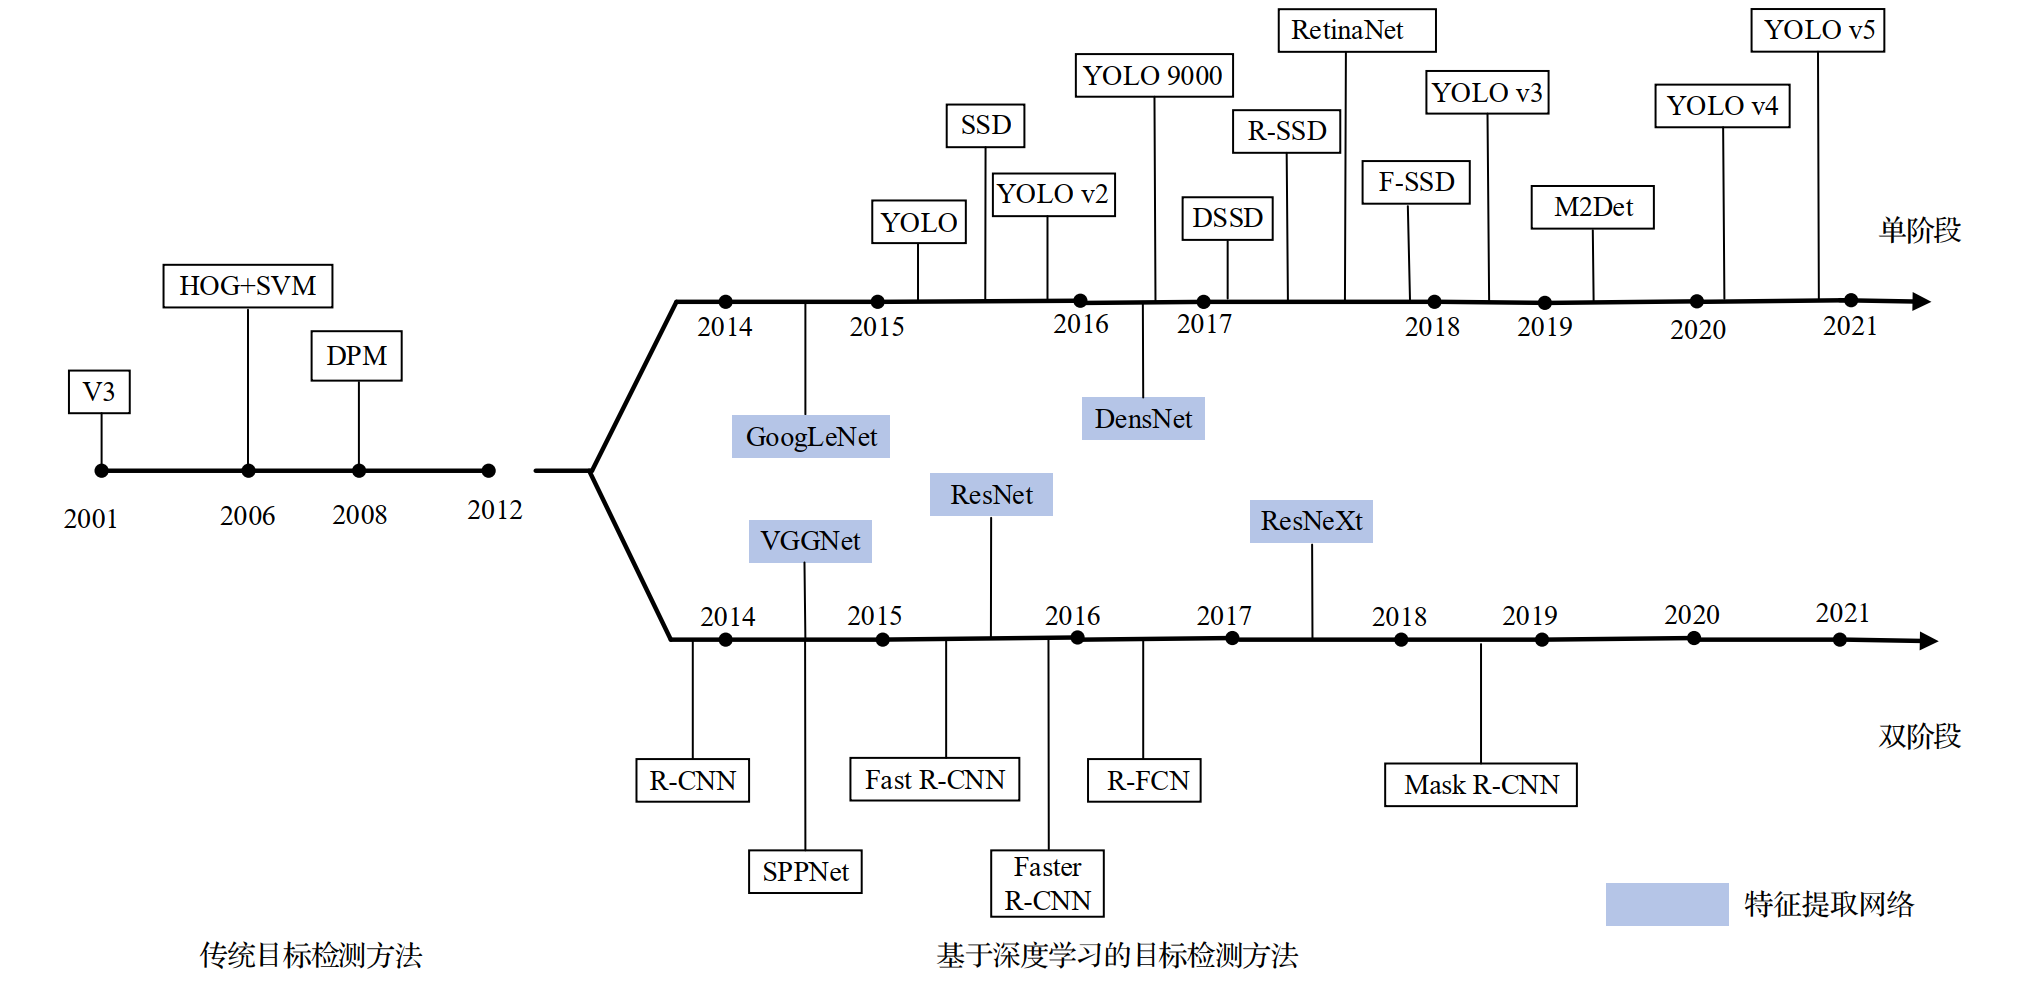
\includegraphics[width=\textwidth]{fig/发展历程.png}
    \caption{跨双栏图片\cite{计算机工程与应用04_fig}}
    \label{fig:发展历程}
\end{figure*}

\section{一级标题}
在大二期间,老师要求按照中大学报来排版课程的综述作业,但我没有找到官方的latex模板;正好在学习latex的使用,于是联系出版社获取了word模板,并参考其制作了此latex模板自用。其中部分内容参考了overleaf上Lee Ruilin制作的模板。

\section{一级标题}
引用文献请在ref.bib中以bib格式粘贴引用,并在文中使用cite命令引用。图片请上传在fig文件夹,下面有图片的使用示例。

\subsection{二级标题}
凑字数凑字数凑字数凑字数凑字数凑字数凑字数凑字数凑字数凑字数凑字数凑字数凑字数凑字数凑字数凑字数凑字数凑字数凑字数凑字数凑字数凑字数凑字数凑字数凑字数凑字数凑字数凑字数凑字数凑字数凑字数凑字数凑字数凑字数凑字数凑字数凑字数凑字数凑字数凑字数凑字数凑字数凑字数凑字数凑字数凑字数凑字数凑字数凑字数凑字数凑字数凑字数凑字数凑字数凑字数凑字数凑字数凑字数凑字数凑字数凑字数凑字数凑字数凑字数凑字数凑字数凑字数凑字数凑字数凑字数凑字数凑字数凑字数凑字数凑字数凑字数凑字数凑字数凑字数凑字数凑字数凑字数凑字数凑字数

\subsubsection{三级标题}
R-CNN在2014年被提出,它通过结合区域提议CNN大幅提高了检测的准确度。模型结构如图\ref{fig:RCNN}所示。尽管R-CNN提升了检测精度,但其处理速度慢且训练复杂,因为需要对每个区域提议独立提取特征,并需要进行多阶段训练,涉及CNN特征提取、SVM分类和边界框回归。

% 单栏图表示例
\begin{center}
    \begin{minipage}{\columnwidth}
        \centering
        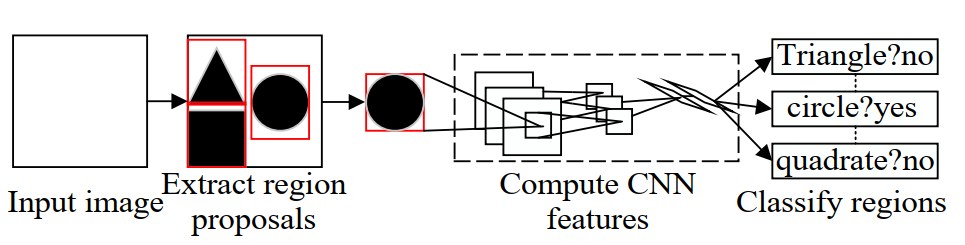
\includegraphics[width=\columnwidth]{fig/RCNN.png}
        \captionof{figure}{单栏图片\cite{计算机工程与应用03_fig}}
        \label{fig:RCNN}
    \end{minipage}
\end{center}


% 跨页表格示例
\end{multicols}

\begin{longtable}{@{}p{0.35\columnwidth}p{0.3\columnwidth}p{0.3\columnwidth}@{}}
    \caption{跨页表格} \label{tab:literature_review} \\
    \toprule
    文献名称 & 研究主题 & 方法/技术 \\
    \midrule
    \endfirsthead
  % 表头在每页顶部重复
    \multicolumn{3}{c}{\tablename\ \thetable{} -- 续上页} \\
    \hline
    文献名称 & 研究主题 & 方法/技术 \\
    \hline
    \endhead

    % 每页底部
    \hline
    \multicolumn{3}{r}{{续下页}} \\
    \hline
    \endfoot

    % 最后一页底部
    \hline
    \endlastfoot

    Rapid object detection using a boosted cascade of simple features & 视觉对象检测 & Integral Image, AdaBoost, 级联分类器 \\ \hline
    Histograms of oriented gradients for human detection & 人体检测 & 线性SVM,HOG描述符 \\ \hline
    % 可以继续添加更多表格内容
\end{longtable}

\begin{multicols}{2}

% 参考文献
\bibliography{ref.bib} % 引用文件名

\end{multicols}

\end{document}